\section{Generative adversarial networks (GANs)}

In this problem, we will implement a generative adversarial network (GAN) that models a high-dimensional data distribution 
$p_{\text{data}}(\bm{x})$, where $\bm{x} \in \Re^{n}$. To do so, we will define a generator $G_{\theta} : \Re^{k} \rightarrow \Re^{n}$; 
we obtain samples from our model by first sampling a $k$-dimensional random vector $\bm{z} \sim \calN(0,I)$ and then returning $G_{\theta}(\bm{z})$.
We will also define a discriminator $D_{\phi} : \Re^{n} \rightarrow (0,1)$ that judges how realistic the generated images 
$G_{\theta}(\bm{z})$ are, compared to samples from the data distribution $x \sim p_{\text{data}}(\bm{x})$. Because its 
output is intended to be interpreted as a probability, the last layer of the discriminator is frequently the \textbf{sigmoid} function,

\begin{equation} \label{eq:4}
    \sigma(x) = \frac{1}{1 + e^{-x}}
\end{equation}

which constrains its output to fall between 0 and 1. For convenience, let $h_{\phi}(\bm{x})$ denote the activation of 
the discriminator right before the sigmoid layer, i.e. let $D_{\phi}(\bm{x}) = \sigma(h_{\phi}(\bm{x}))$. The values 
$h_{\phi}(\bm{x})$ are also called the discriminator’s \textbf{logits}.

There are several common variants of the loss functions used to train GANs. They can all be described as a 
procedure where we alternately perform a gradient descent step on $L_{D}(\phi;\theta)$ with respect to $\phi$ to train 
the discriminator $D_{\phi}$, and a gradient descent step on $L_{G}(\theta;\phi)$ with respect to $\theta$ to train the 
generator $G_{\theta}$:

\begin{equation} \label{eq:5}
    \min\limits_{\phi} L_{D}(\phi; \theta), \hspace{5em} \min\limits_{\theta} L_{G}(\theta; \phi).
\end{equation}

In lecture, we talked about the following losses, where the discriminator’s loss is given by

\begin{equation} \label{eq:6}
    L_{D}(\phi; \theta) = - \E_{\bm{x} \sim p_{\text{data}}(\bm{x})} [\log D_{\phi}(\bm{x})] - \E_{\bm{z}\sim\calN(0,I)}[\log\left(1-D_{\phi}\left(G_{\theta}\left(\bm{z}\right)\right)\right)]
\end{equation}

and the generator’s loss is given by the \textbf{minimax loss}

\begin{equation} \label{eq:7}
    L_{G}^{\text{minimax}}(\theta;\phi) = \E_{\bm{z} \sim \calN(0,I)}[\log\left(1 - D_{\phi}\left(G_{\theta}\left(\bm{z}\right)\right)\right)]
\end{equation}

\begin{enumerate}[label=(\alph*)]
    \item \input{02-gan/01-minmax}

    \item \points{2b} Because of this vanishing gradient problem, in practice, $L_{G}^{\text{minimax}}$ is typically replaced with
    the \textbf{non-saturating loss} 

    \begin{equation} \label{eq:9}
        L_{G}^{\text{non-saturating}}(\theta;\phi) = -E_{\bm{z}\sim\calN(0,I)}[\log D_{\phi}\left(G_{\theta}\left(\bm{z}\right)\right)]
    \end{equation}

    To turn the non-saturating loss into a concrete algorithm, we will take alternating gradient steps on Monte Carlo 
    estimates of $L_D$ and $L_{G}^{\text{non-saturating}}$:

    \begin{equation} \label{eq:10}
        L_D(\phi; \theta) \approx - \frac{1}{m} \sum\limits_{i=1}^{m} \log D_{\phi}\left(\bm{x}^{(i)}\right) - \frac{1}{m}\sum\limits_{i=1}^{m} \log\left(1-D_{\phi}\left(G_{\theta}\left(\bm{z}^{(i)}\right)\right)\right)
    \end{equation}

    \begin{equation} \label{eq:11}
        L_{G}^{\text{non-saturating}}(\theta;\phi) \approx - \frac{1}{m} \sum\limits_{i=1}^{m} \log D_{\phi}\left(G_{\theta}\left(\bm{z}^{(i)}\right)\right)
    \end{equation}

    where $m$ is the batch size, and for $i = 1,...,m$, we sample $\bm{x}^{(i)} \sim p_{\text{data}}(\bm{x})$ and $\bm{z}^{(i)} \sim \calN(0,I)$.

    Implement and train a non-saturating GAN on Fashion MNIST for one epoch. Read through \texttt{main.py}, 
    and in \texttt{submission/gan.py}, implement the \texttt{loss\_nonsaturating\_g} and \texttt{loss\_nonsaturating\_d} functions. 

    To train the model, execute:
    \begin{verbatim}
        python main.py --model gan --out_dir gan_nonsat
    \end{verbatim}  

    For GPU acceleration run run the command below. \textbf{Note:} we are not supporting MPS GPUs as it trains slower than CPU-enabled training on Apple Silicon devices.
    \begin{verbatim}
        python main.py --model gan --out_dir gan_nonsat --device gpu
    \end{verbatim} 
    
    You may monitor the GAN’s output in the \texttt{gan\_nonsat} directory. Note that because the GAN is only trained for one epoch, 
    we cannot expect the model’s output to produce very realistic samples, but they should be roughly recognizable as clothing items.

    \textbf{Hint}: Note that $1-\sigma(x) = \sigma(-x)$.

    For reference, the generated examples should look similar to the image below:
    \begin{figure}[h]
        \centering
        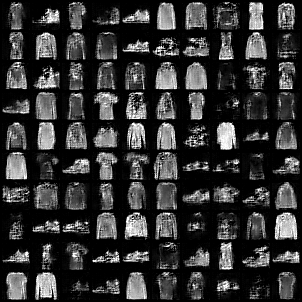
\includegraphics[width=0.5\textwidth]{./figures/gan_nonsat_0900}
    \end{figure}

\end{enumerate}
